\documentclass[a4paper,10pt]{article}
\usepackage[utf8]{inputenc}
\usepackage{geometry} 	%pour les marges
\usepackage{color} %pour la definition de nouvelles couleurs
\usepackage{graphicx} %pour ajouter des images 
\usepackage[final]{pdfpages} 
\usepackage[francais]{babel} % ``Franciser '' le document
\usepackage{lscape}
\usepackage	
  [colorlinks=false, urlcolor=red, breaklinks, pagebackref, citebordercolor={0 0 0}, 
  filebordercolor={0 0 0}, linkbordercolor={0 0 0}, pagebordercolor={0 0 0}, 
  runbordercolor={0 0 0}, urlbordercolor={0 0 0}, pdfborder={0 0 0}]
	{hyperref} % Ajouter le package des lien redirigeant sans les encadrer 
\usepackage{eurosym}
\usepackage{dirtree}
\usepackage{comment}

%couleurs pour les morceaux de code
\definecolor{codegreen}{rgb}{0,0.6,0}
\definecolor{codered}{rgb}{1,0.1,0.2}
\definecolor{codegray}{rgb}{0.5,0.5,0.5}
\definecolor{codepurple}{rgb}{0.58,0,0.82}
\definecolor{backcolour}{rgb}{0.95,0.95,0.92}
 

%modificaion des marges
\geometry{hmargin=2.5cm,vmargin=3cm}


%opening
\title{Architecture Logicielle : UML Reverse}

\title{\bfseries Document Architecture Logicielle \\Projet UML Reverse}
\geometry{hmargin=2.5cm,vmargin=3cm}
\begin{document}
\maketitle
\begin{center}
\begin{tabular}{ll}
  Version~: & 0.1\\[.5em]
  Date~: & \date{\today}\\[.5em]
  Rédigé par~:  & Yohann \textsc{Henry}\\
		& Nabil \textsc{Belkhous}\\[.5em]   
		& Stephen \textsc{Cauchois}\\
		& Anthony \textsc{Godin}\\
		& Florian \textsc{Inchingolo}\\
		& Saad \textsc{Mrabet}\\
		& Nicolas \textsc{Meniel}\\
\end{tabular}
\end{center}

\newpage
\begin{center}
    \section*{Mises à jour}
    \begin{tabular}{|l|l|p{8cm}|}
        \hline{\textbf{Version}} & {\textbf{Date}} & {\textbf{Modifications réalisées}}\\\hline
        {0.2} & {22/01/2016} & {Architecture refaite dans l'intégralité}\\\hline
        {0.1} & {14/01/2016} & {Première version}\\\hline
    \end{tabular}
\end{center}

%Table of contents
\newpage
\tableofcontents
\newpage


\section{Objectif}
Ce document représente la structure générale du logiciel et les modèles de conception mis en oeuvre pour le réaliser.
Il est destiné aux membres de l'équipe de développment, notamment aux concepteurs, ainsi qu'aux superviseurs du projet.

\section{Les technologies utilisées}
Nous allons utiliser différentes technologies pour la construction du projet.
\newline
Le projet est développé en java 1.8.
Le projet utilise :
\begin{itemize}
 \item \emph{Dot} : Un outil permettant de calculer la position idéale des entités et des relations d'un graphe. 
 Cela nous évite la partie mathématique pour le placement des relations qui aurait pu s'avérer un risque majeur.
 \item \emph{JUnit} : Framework pour valider chaque classe par le biais de tests unitaires.
 \item \emph{Maven} : Un outil pour la gestion des dépendances de l'application.
 \item \emph{Antlr} : Un parser dans lequel nous pourrons définir les grammaires pour l'extraction des données d'un fichier java ou plantUml.
 \item \emph{openJFX} : Une bibliothèque libre graphique parfaite pour ce projet. La bibliothèque permet d'associer à une entité du CSS,
			ce qui simplifie fortement notre travail.
 \item \emph{SceneBuilder} : Logiciel permettant de créer des vus de façon ergonomique en drag and drop. Les vus sont créées en fxml.  
\end{itemize}

\section{Fonctionnement général}
  \begin{center}
      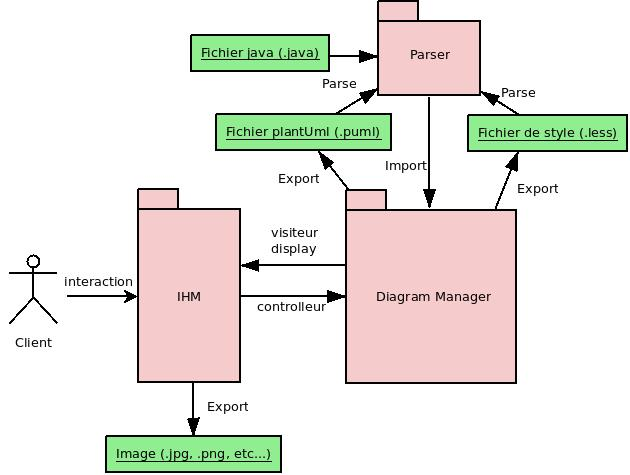
\includegraphics[width=\textwidth]{Image/generalDal.jpg}
  \end{center}
  L'architecture est construite suivant le modèle MVC. Cela nous permet de séparer les responsabilités des classes.
 
\section{Organisation des paquetages}

  \dirtree{%
    .1 src.
    .2 main\DTcomment{Contient la classe d'entrée du logiciel}.
    .3 UmlReverseApp.java.
    .2 model.
    .3 diagram\DTcomment{Modèlise un diagramme en objet}.
    .4 clazz.
    .5 visitor\DTcomment{Permet le parcourt du diagramme de classe}.
    .4 usecase.
    .5 visitor\DTcomment{Permet le parcourt du diagramme de cas}.
    .4 visitor\DTcomment{Visiteurs globaux. Choisi d'appeller un visiteur en particulier selon le type de diagramme}.
    .3 io.
    .4 antlr.
    .2 ui.
    .3 view\DTcomment{Contient les vues principales de l'application avec leurs contrôleurs}.
    .3 component\DTcomment{Contient les composants utilisés dans la vue}.
    .4 clazz.
    .4 usecase.
    .4 common.
  }

  \section{Paquetage model}
    Ce package contient l'intégralité du modèle. Voir le diagramme de classe en annexe (diagramClassModel).
    
   \newpage
  \section{Paquetage ui}
    L'application s'appuie sur la structure JavaFX avec la classe applicative UmlReverseApp qui est composée d'un stage qui en suivant
    la hiérarchie JavaFX nous ammène au BorderPane. Le BorderPane nous servira de base pour les différents éléments de notre application,
    tel qu'une TreeFileManagerView, une MenuBar, un IDiagramEditor et un IDiagramMenu.
    \begin{center}
	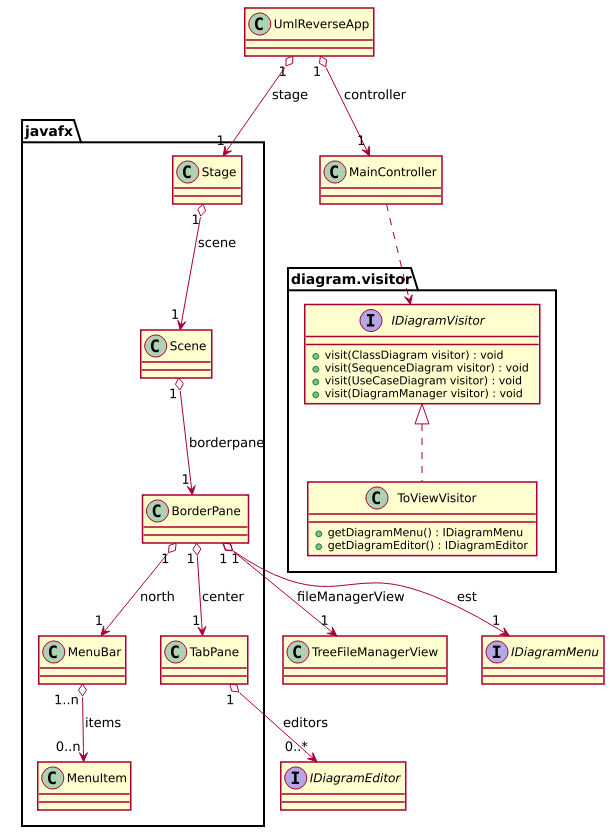
\includegraphics[width=10cm]{Image/Vue.png}
    \end{center}
  
    Ce paquetage contient toutes les classes utilisées pour gérer la vue. Ces classes sont toujours associées à un contrôleur.
    Les vues sont codées en fxml grâce à un logiciel de construction de fxml (SceneBuilder). Chaque contrôleur aura le même nom
    que la vue associée avec le mot ``Controller'' ajouté à la fin.
    ui contient 2 paquetages :
    \begin{itemize}
    \item view : Contient les différentes vues intégrées dans l'application. Le paquetage contient également tous les contrôleurs associés à leur vue.
    \item component : Contient toutes les classes utilisées pour construire les vues. Ce sont leurs composants.
    \end{itemize}
    L'application graphique est l'association de plusieurs vues dans un BorderPane.
    
    \begin{center}
	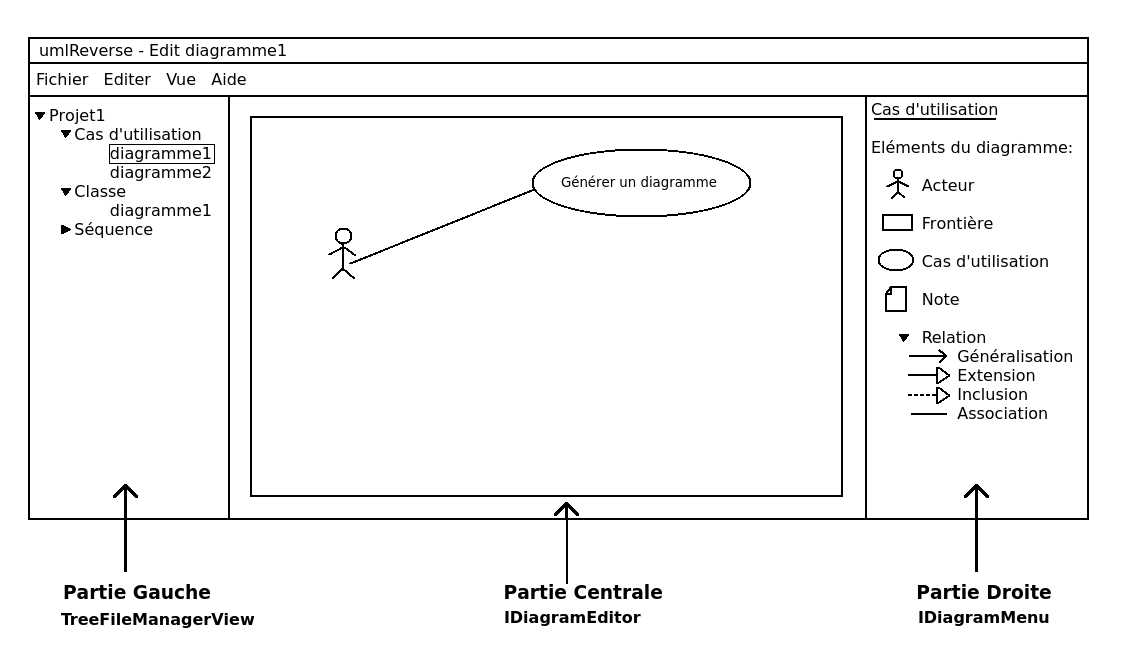
\includegraphics[width=\textwidth]{Image/maquette.png}
    \end{center}

  \subsection{La partie gauche}
    La partie gauche présente la liste des projets disponibles et des diagrammes qu’ils contiennent, et permet de naviguer entre eux. 
    Cette tâche est accomplie par un modèle qui gère les fichiers, accompagné d’une vue hiérarchique constructible à partir de ce modèle.
    
    \begin{center}
	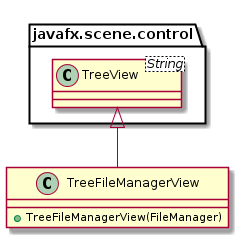
\includegraphics[width=4cm]{Image/partieGaucheVue.png}
    \end{center}
  \subsection{La partie centrale}
    La partie centrale sert à éditer graphiquement un diagramme. La vue principale de cette partie est codée en javafx avec 
    des classes tel que ObjectEntityGraphic.java qui dessine une classe. Et
    associé à son contrôleur ObjectEntityGraphicController.java par exemple.\\
    
    \textbf{\underline{Explication}}: Toutes les classes qui finissent par Graphic sont des réprésentations graphiques des élements du modèle. Elles contiennent
    des écouteurs de souris sur elles mêmes pour pouvoir permettre aux utilisateurs de les modifier ce qui modifiera le modèle directement.
    La modification du modèle modifie obligatoirement la vue du diagramme (les éléments graphiques donc) grâce à des écouteurs sur le modèle.
    \newpage
    \subsubsection{Editeur de diagramme}
	La partie MVC a été volontairement omise pour éviter de surcharger le diagramme de classe. Elle sera 
	par contre implémenté dans les parties prévues.\\
	Dans les diagrammes ci contre les contrôleurs controleront les actions de IDiagramEditor.\\
	Les editeurs de seront suffixé d'Edit, il y en aura pour chaque entié que ce soit un ObjectEntityGraphic ou
	une Relation. Des classes pour éditer seront disponible elles seront préfixé par Dialog et suffixé par
	Edit.
	\subsubsection{Paquetages}
	
	  \begin{center}
	      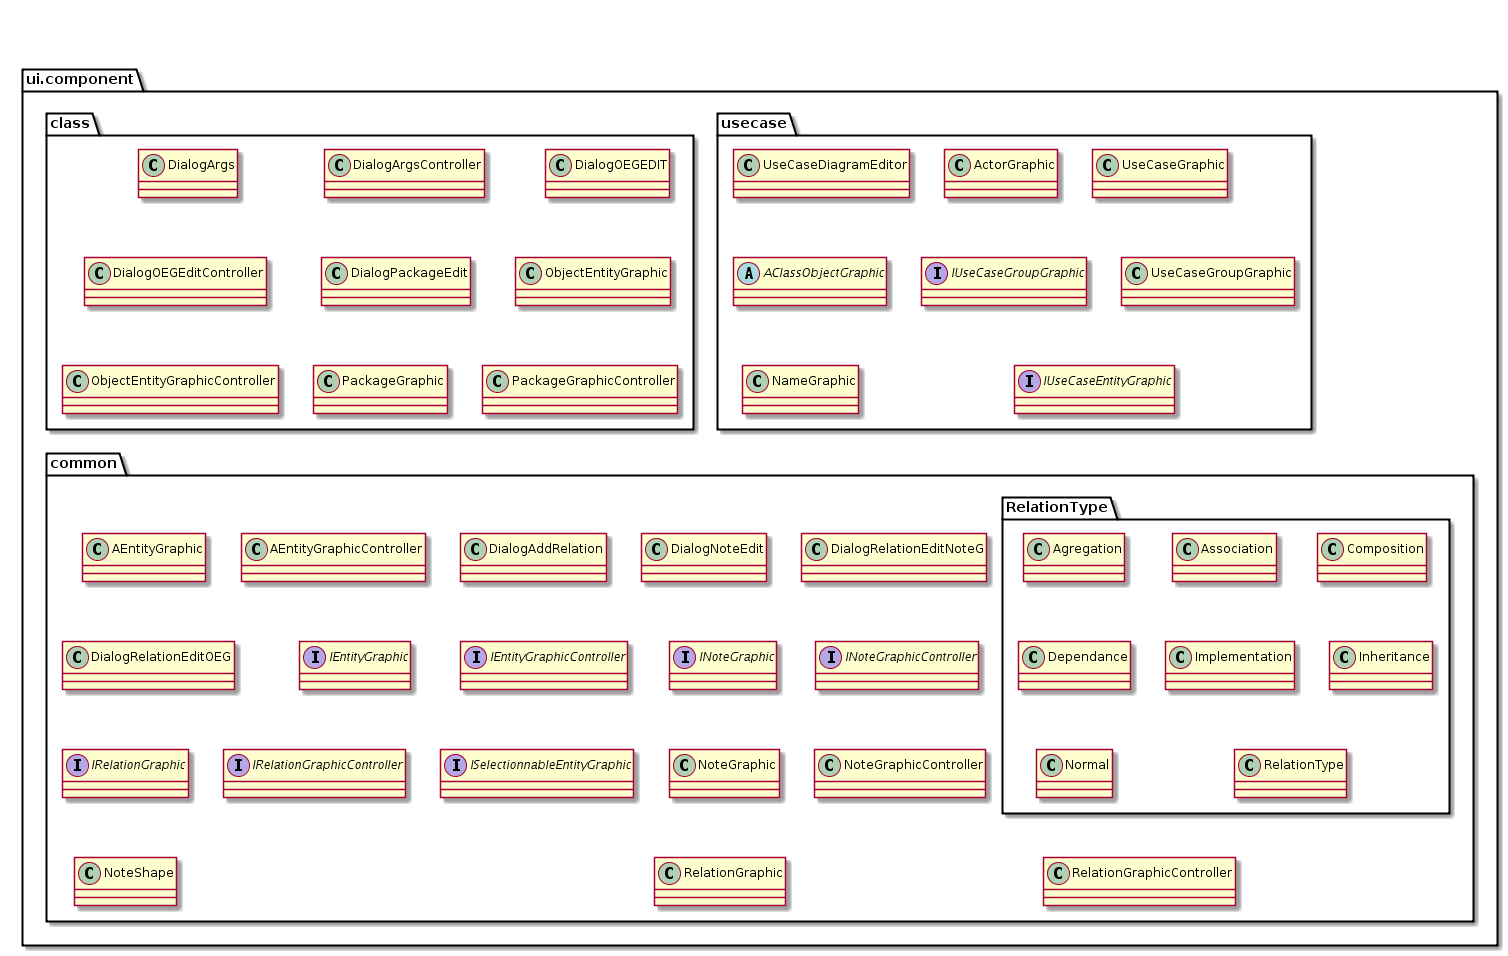
\includegraphics[width=\textwidth]{DiagrammesVueVersion1erLivrable/DiagramEditor_EntityPackage3.png}
	  \end{center}
	  Voici toutes les entités que nous qui sont présentes dans nos packages. Elles sont ici représenté sans relation.
	  \newpage
	\paragraph{Package view }
	\begin{center}
	    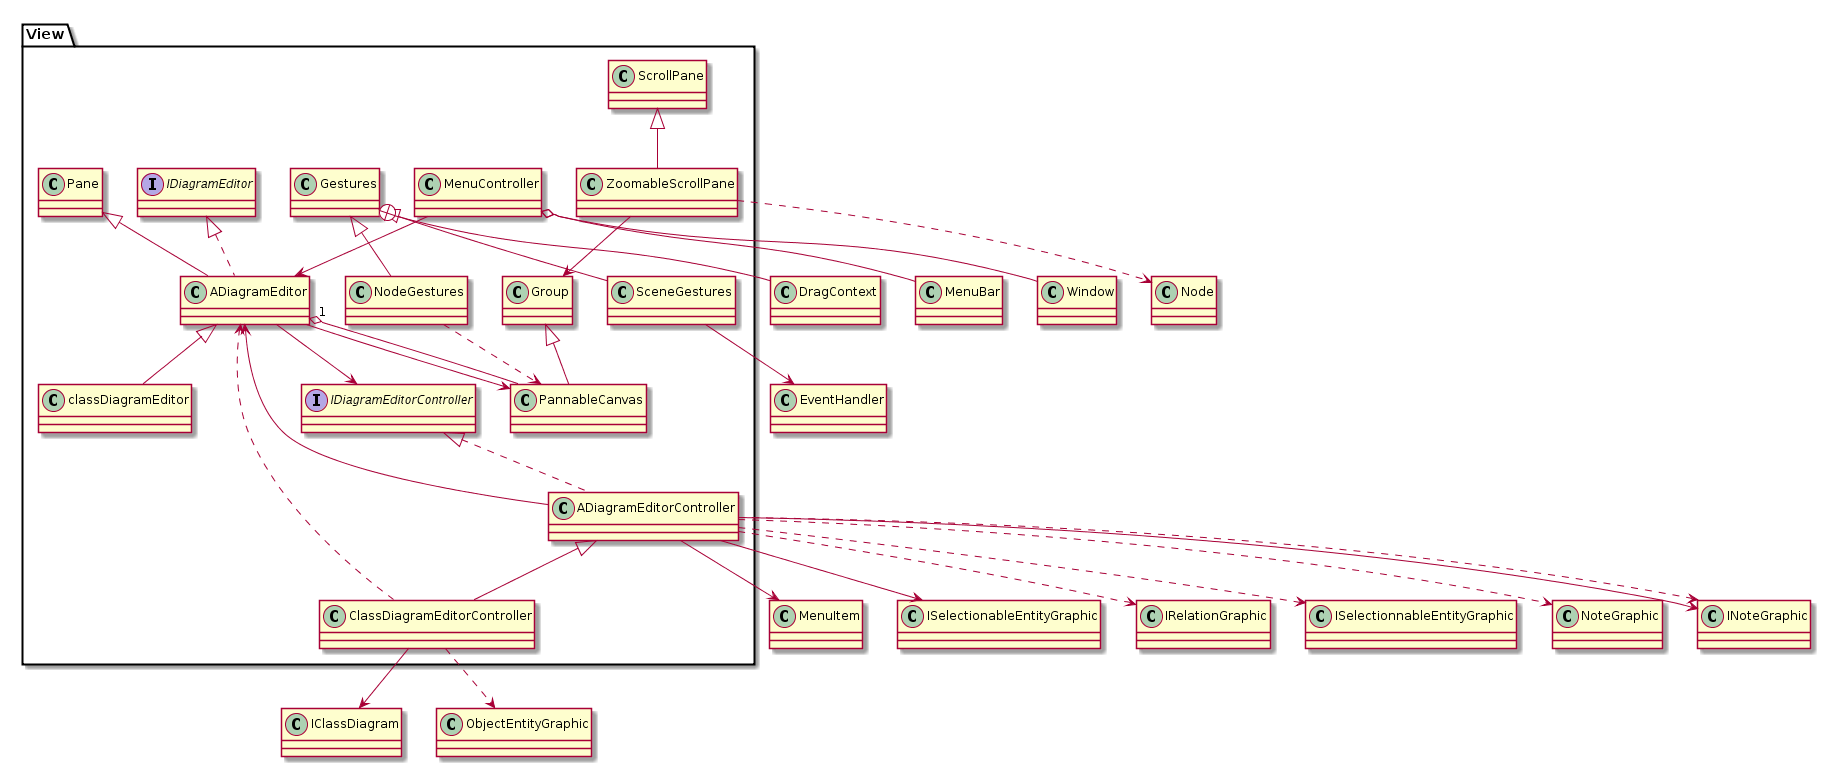
\includegraphics[width=\textwidth]{DiagrammesVueVersion1erLivrable/viewsimplifie.png}
	\end{center}
	Dans ce diagramme on peut voir le package view représentant la base de notre application graphic, avec les différentes classes permettant
	le zoom et le drag and drop.
	
	\newpage
    \paragraph{Package common }
	  \begin{center}
	      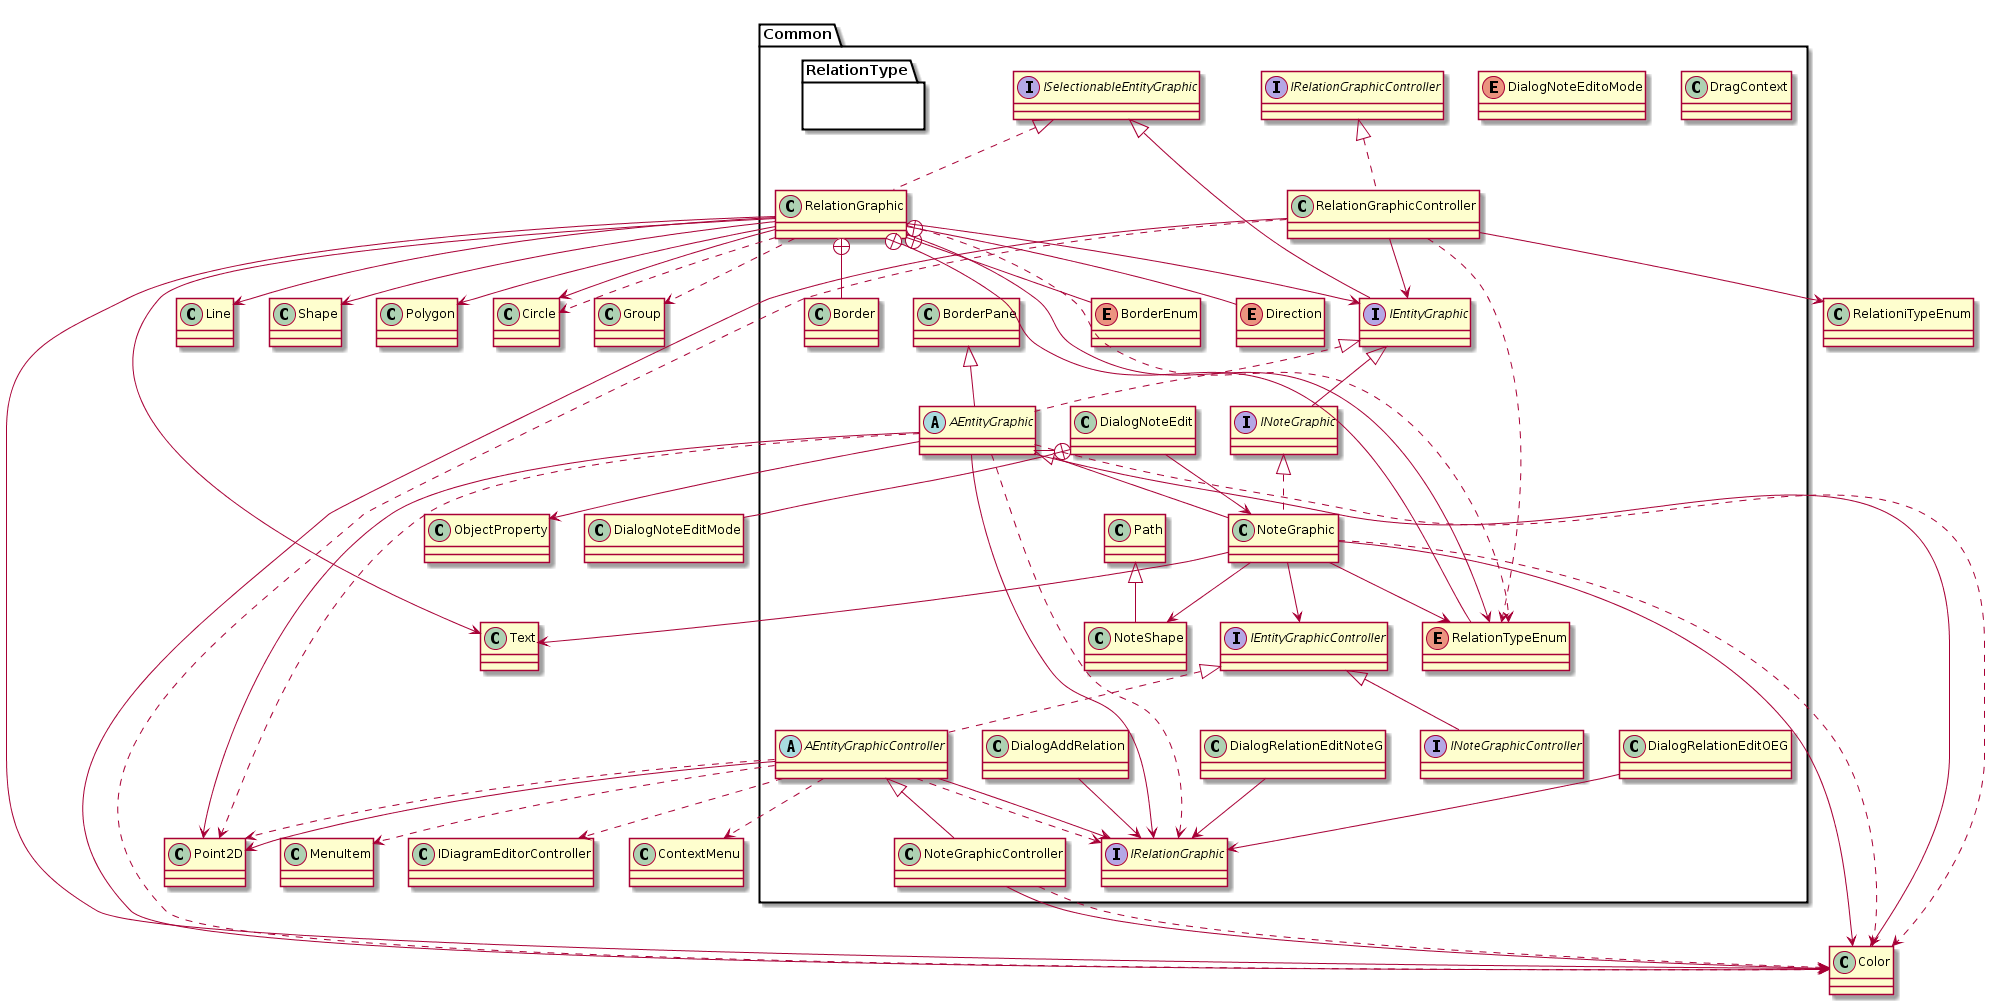
\includegraphics[width=\textwidth]{DiagrammesVueVersion1erLivrable/CommonSimplifie.png}
	  \end{center}
	  Dans ce diagramme on peut voir la représentation des entités permettant la création et l'édition de note ou de relation. La gestion du menu
	  contextuel est aussi présente dans ce diagramme.
	  \newpage
    \paragraph{package clazz}
	  \begin{center}
	      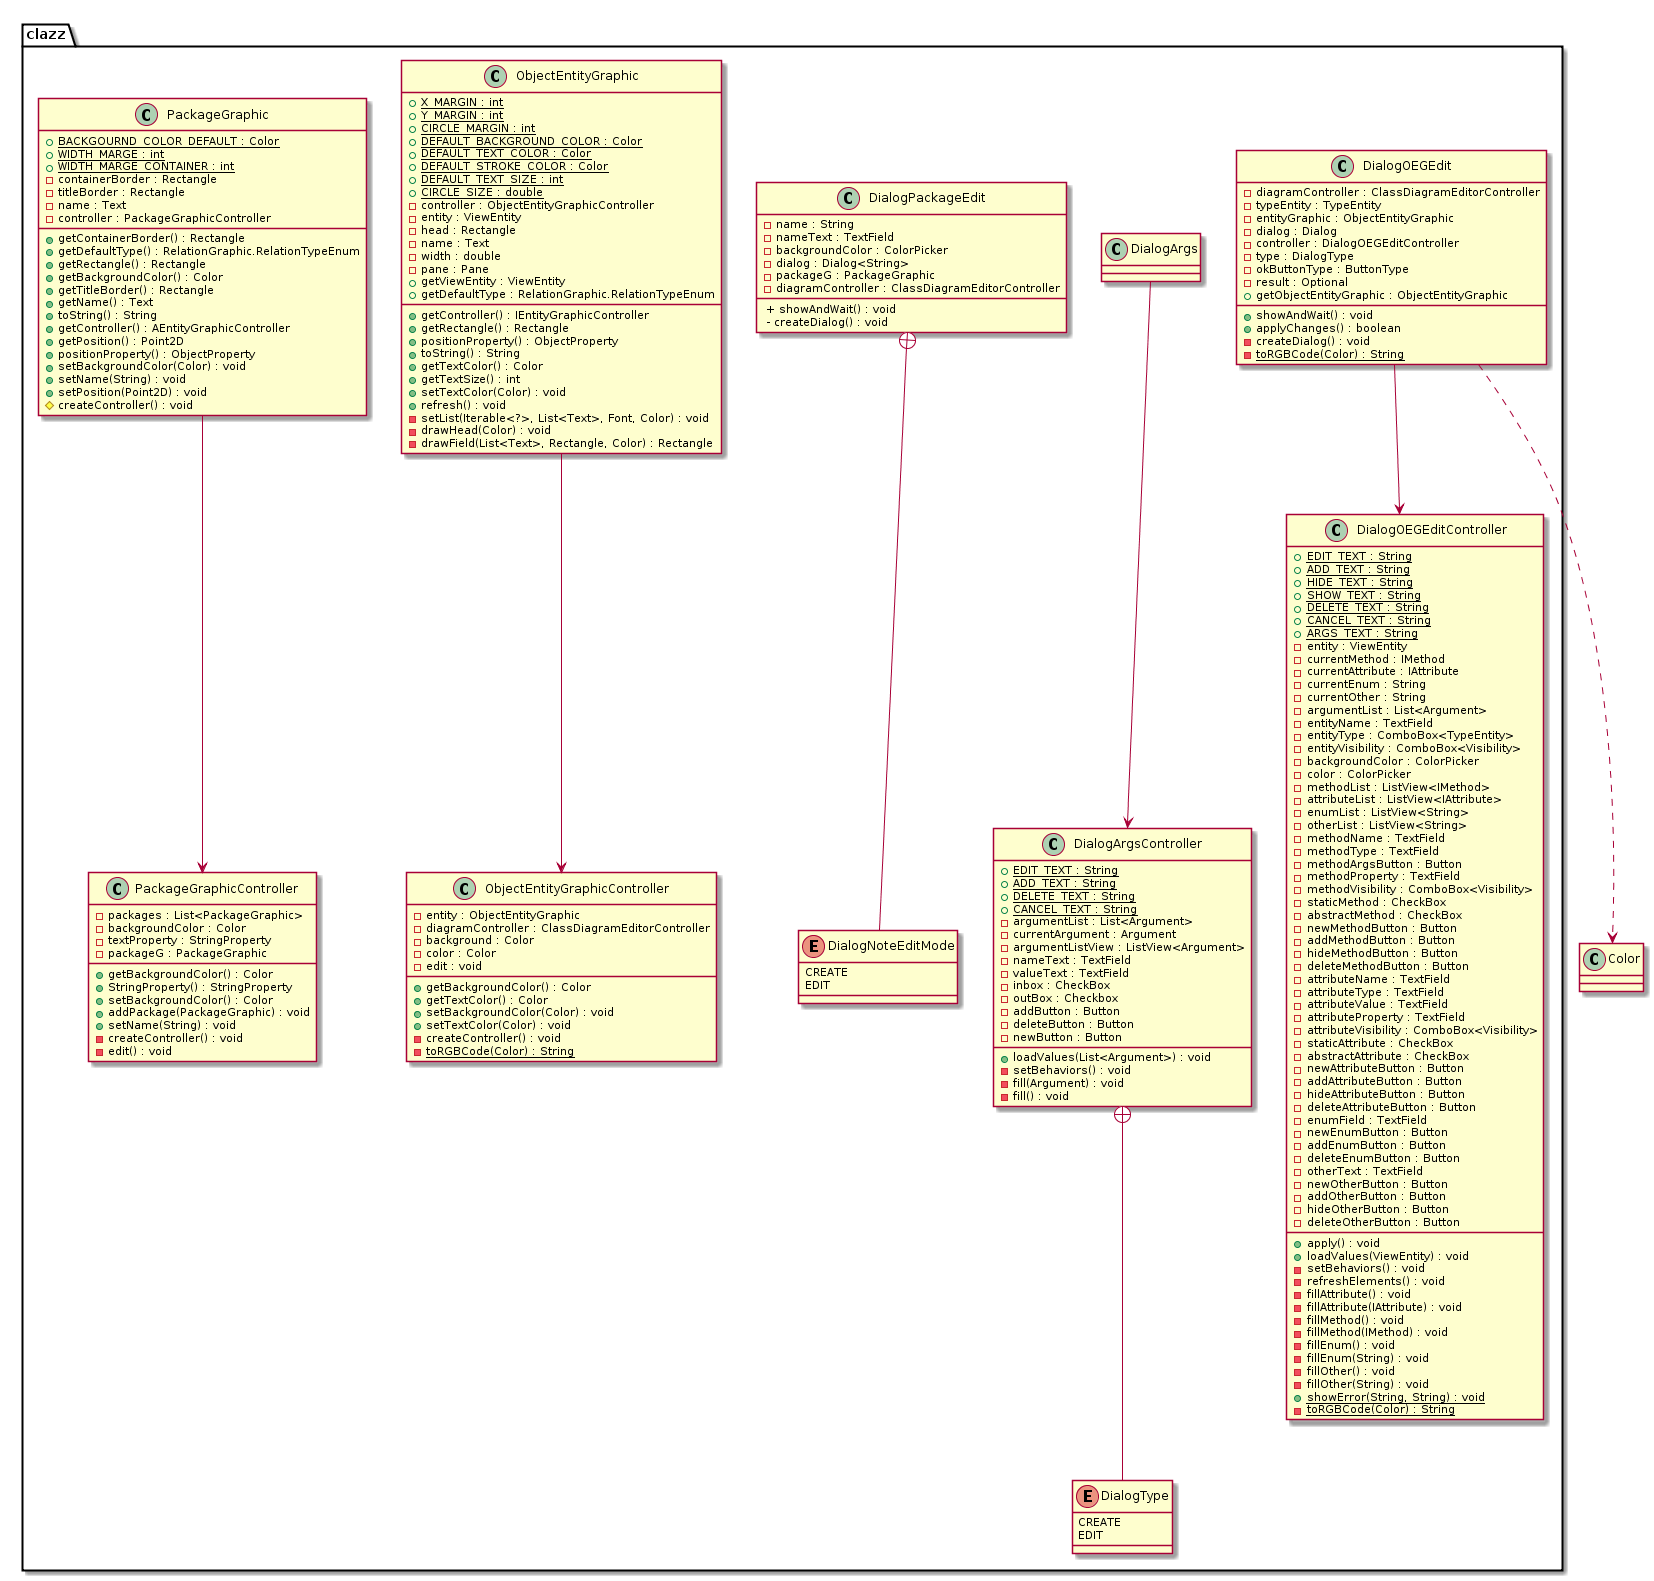
\includegraphics[width=\textwidth]{DiagrammesVueVersion1erLivrable/clazz.png}
	  \end{center}
	  Dans ce diagramme il y a toutes les entités spécifique aux diagrammes de classes, on peut donc y trouver les package ainsi que les ObjectEntity 
	  qui représentent les différent type de classes, interface etc... que l'ont peut dessiner
	  
   
    \subsubsection{Explications}
	\begin{center}
	  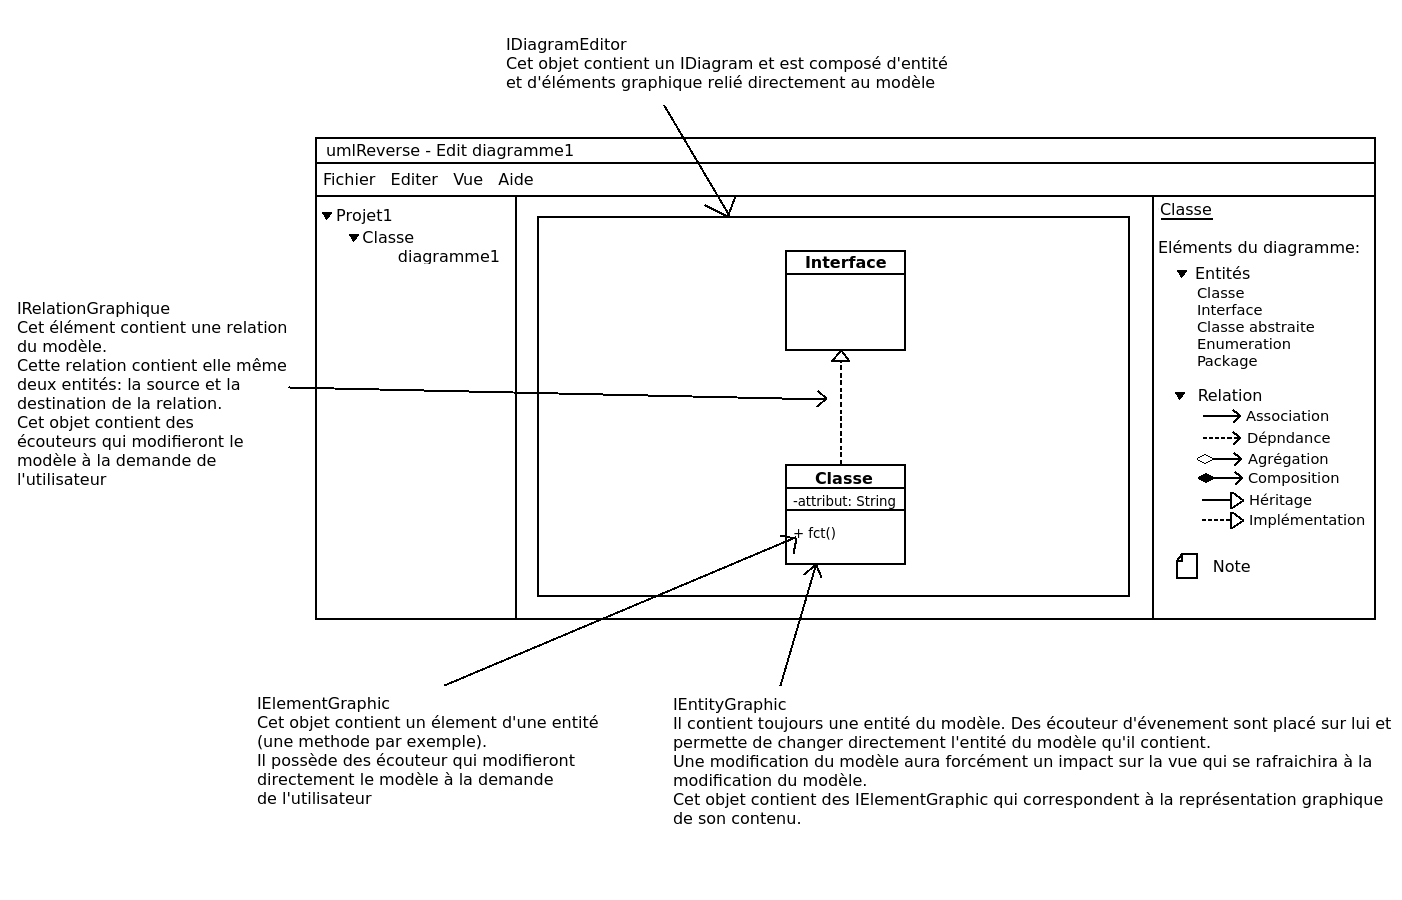
\includegraphics[width=\textwidth]{Image/demonstration.png}
	\end{center}
      
  \subsection{La partie droite}
    \subsubsection{Déroulement}
      Quand un utilisateur séléctionne un diagramme l'action fait appel au contrôleur qui va passer par l'interface IDiagram du modèle et le visiteur 
      permet de déterminer le type de diagramme selectionné.
      L'interface IDiagramMenu nous permet d'ajouter des entités et des relations dans un diagramme grâce au contrôleur qui gère les actions.
       
    \subsubsection{Diagramme de classe} 
          \begin{center}
	     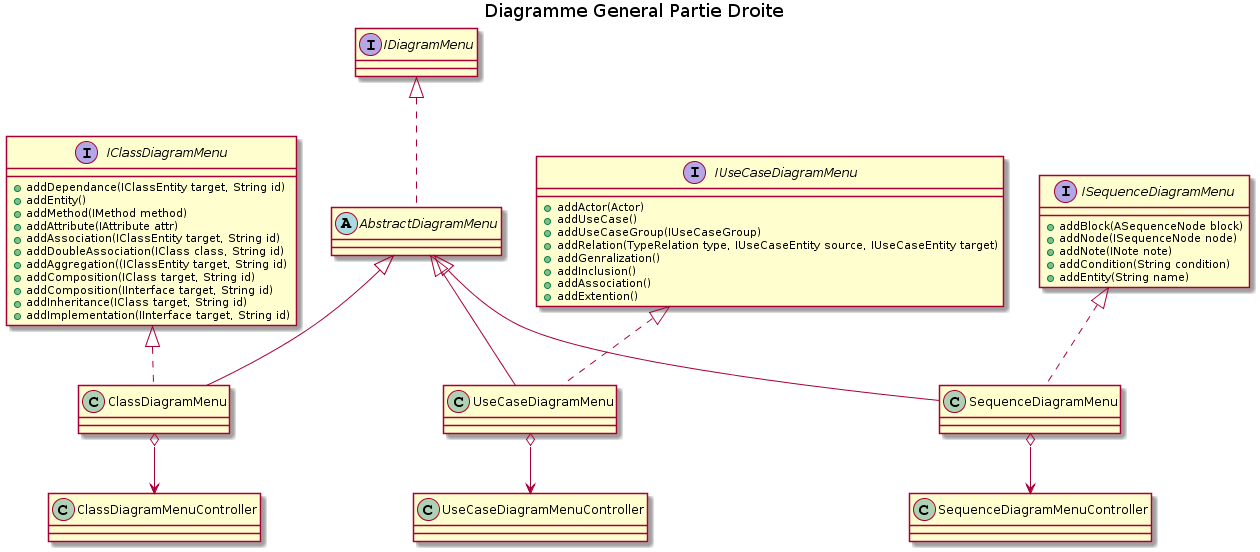
\includegraphics[width=15cm]{Image/DiagramGenrDroite.png}
          \end{center}
          
\section{Paquetage main}
    Contient la classe qui lance l'application. C'est le point d'entrée. Il charge les différentes vues du paquetage ui.view en les rassemblant toutes dans un BorderPanel.
    
\section{Diagramme de Séquence}
  \subsection{Ouverture de l'application}
  \begin{center}
	     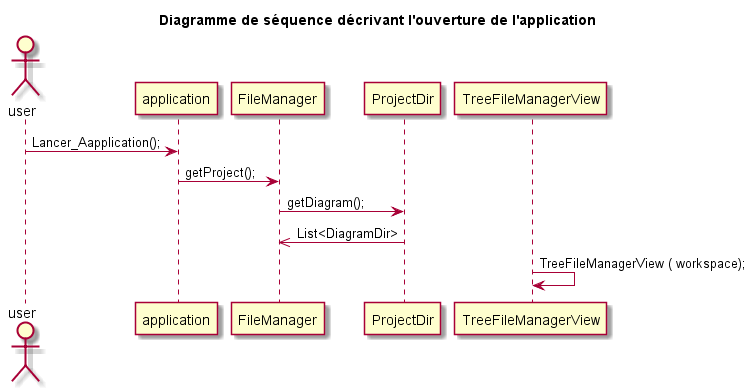
\includegraphics[width=14cm]{Image/Diag_Seq_Open.png}
   \end{center}
    
   \subsection{Chargement d'un diagramme dans la vue}
   \begin{center}
	     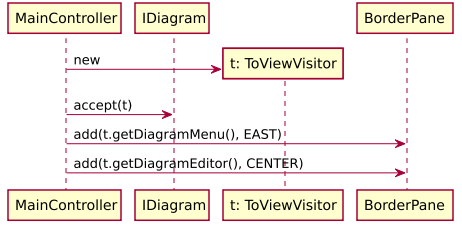
\includegraphics[width=8cm]{Image/uiupdate.png}
   \end{center}
   
   \subsection{Chargement d'un fichier java}
    \begin{center}
	     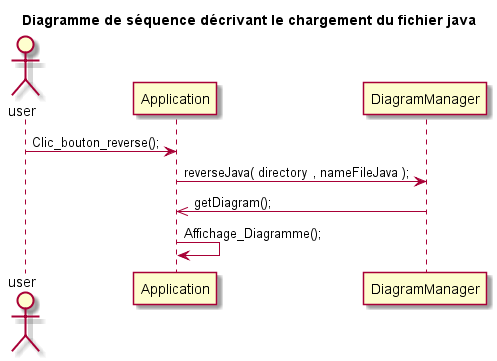
\includegraphics[width=10cm]{Image/Charge_File_Java.png}
    \end{center}
  
\section{Extensibilité}
  L'architecture a été pensé de façon à vérifier l'exigence EXF\_70 (code modulaire, ajout de nouvelles fonctionnalités possible dans le code).
  \paragraph{Modèle}
    Le modèle a été pensé à facilement ajouter de nouveau type de diagramme. Pour ce faire le gestionnaire de diagramme ne se soucis pas du type de diagramme.
    La plupart des actions demandées sur un diagramme de manière extérieur au modèle se font par le biais des visiteurs. Pour ajouter un nouveau
    type de diagramme il suffit de créer une nouvelle classe qui implémente IDiagram et de mettre à jour les visiteurs globaux.
  \paragraph{Partie gauche de l'application}
    Les différentes classes créées peuvent être héritées afin d'étendre leurs fonctionnalitées ainsi que d'ajouter de nouveaux types de diagramme. 
    L'architecture des dossiers d'un projet a été pensée afin que l'ajout de nouveau type de fichier pour la sauvegarde des diagrammes
    soit simple sans rendre les projets de cette version obsolète.
  \paragraph{IDiagramEditor}
    Tout d'abord, l'ajout de nouveau type de diagramme a été pensé de façon à être possible et facile à implémenter. 
    Pour se faire, il suffit d'ajouter dans le IDiagramEditor une 
    nouvelle classe XXXDiagramEditor. Cette nouvelle classe peut hériter ADiagramEditor si le nouveau type de diagramme peut posséder des notes.
    L'implémentation de celle ci sera déjà implémentée.
    Les classes présentes dans le paquetage view.component.common sont des classes qui peuvent être utilisées dans n'importe qu'elle type de diagramme. Ce
    sont généralement des classes abstraites qui font une partie du travail. Ce qui évite de tous refaire à chaque fois.
    
  \paragraph{IDiagramMenu}
    Cette partie peut aussi facilement ajouter des nouveaux types de diagrammes. Il suffit de rajouter un nouveau type de menu et d'implémenter la bonne interface.



\begin{comment}
  \subsection{model}
  Ce package contient l'intégralité du modèle. Il contient tous les packages et classes pour le travail métier.
  \subsubsection{util}
  Le code commun à tous les diagrammes
  \begin{center}
      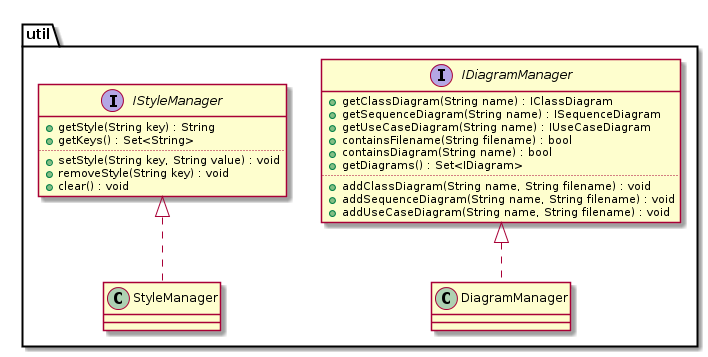
\includegraphics[width=\textwidth]{Image/util2.png}
  \end{center}
  \begin{landscape}
      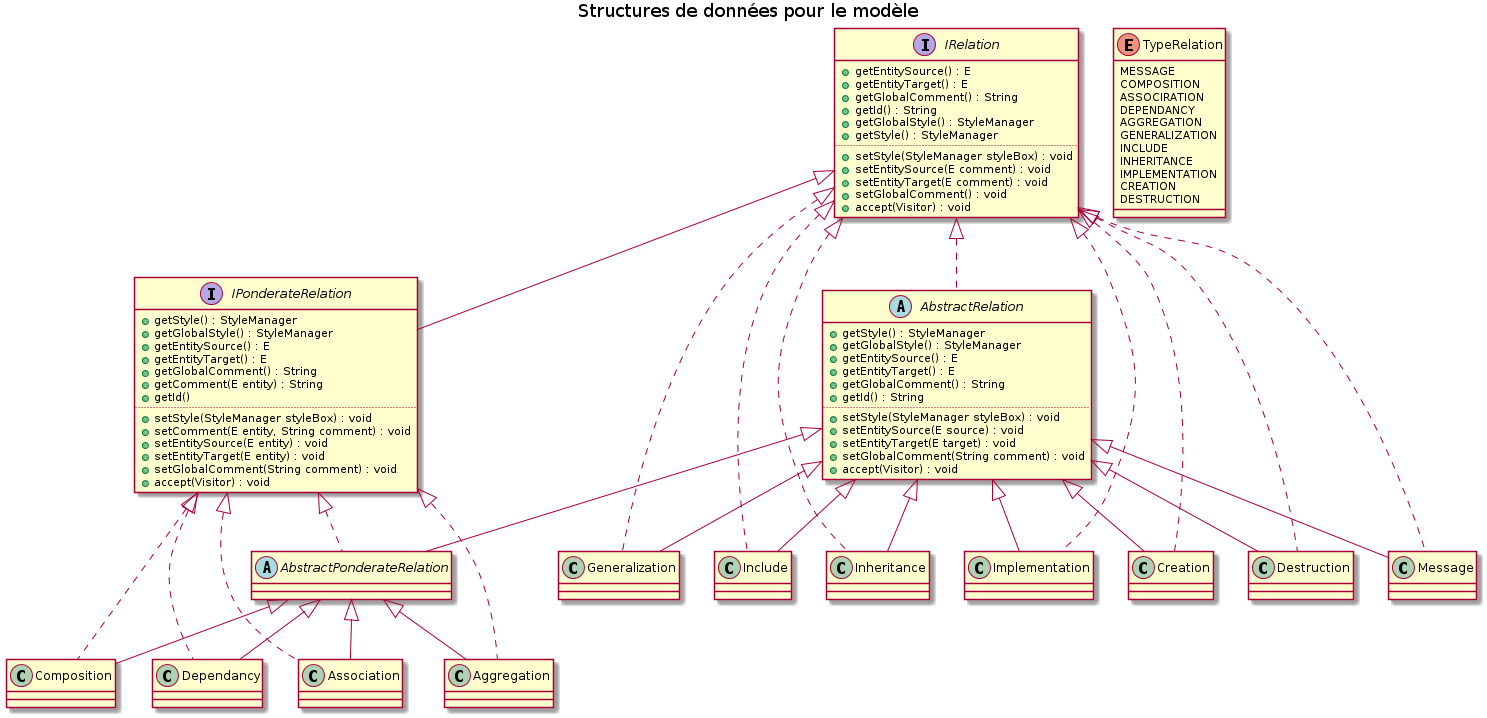
\includegraphics[height=12cm]{Image/utilDiagramme.png}
  \end{landscape}
  Ce package contient l'intégralité du code commun à chaque diagramme. 
  C'est aussi ici qu'on trouve la définition des boîtes de style.
  \subsubsection{visitor}
  Les visiteurs permettent l'ajout d'opérations homogènes à des entités d'un modèle sans couplage.
  \begin{center}
      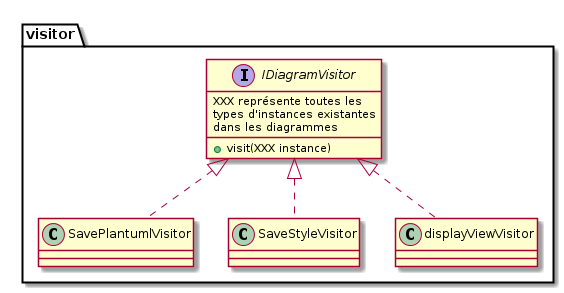
\includegraphics[width=\textwidth]{Image/visitor.png}
  \end{center}
  Ce package contient les visiteurs des diagrammes.
  \subsubsection{classDiagram}
  \begin{center}
      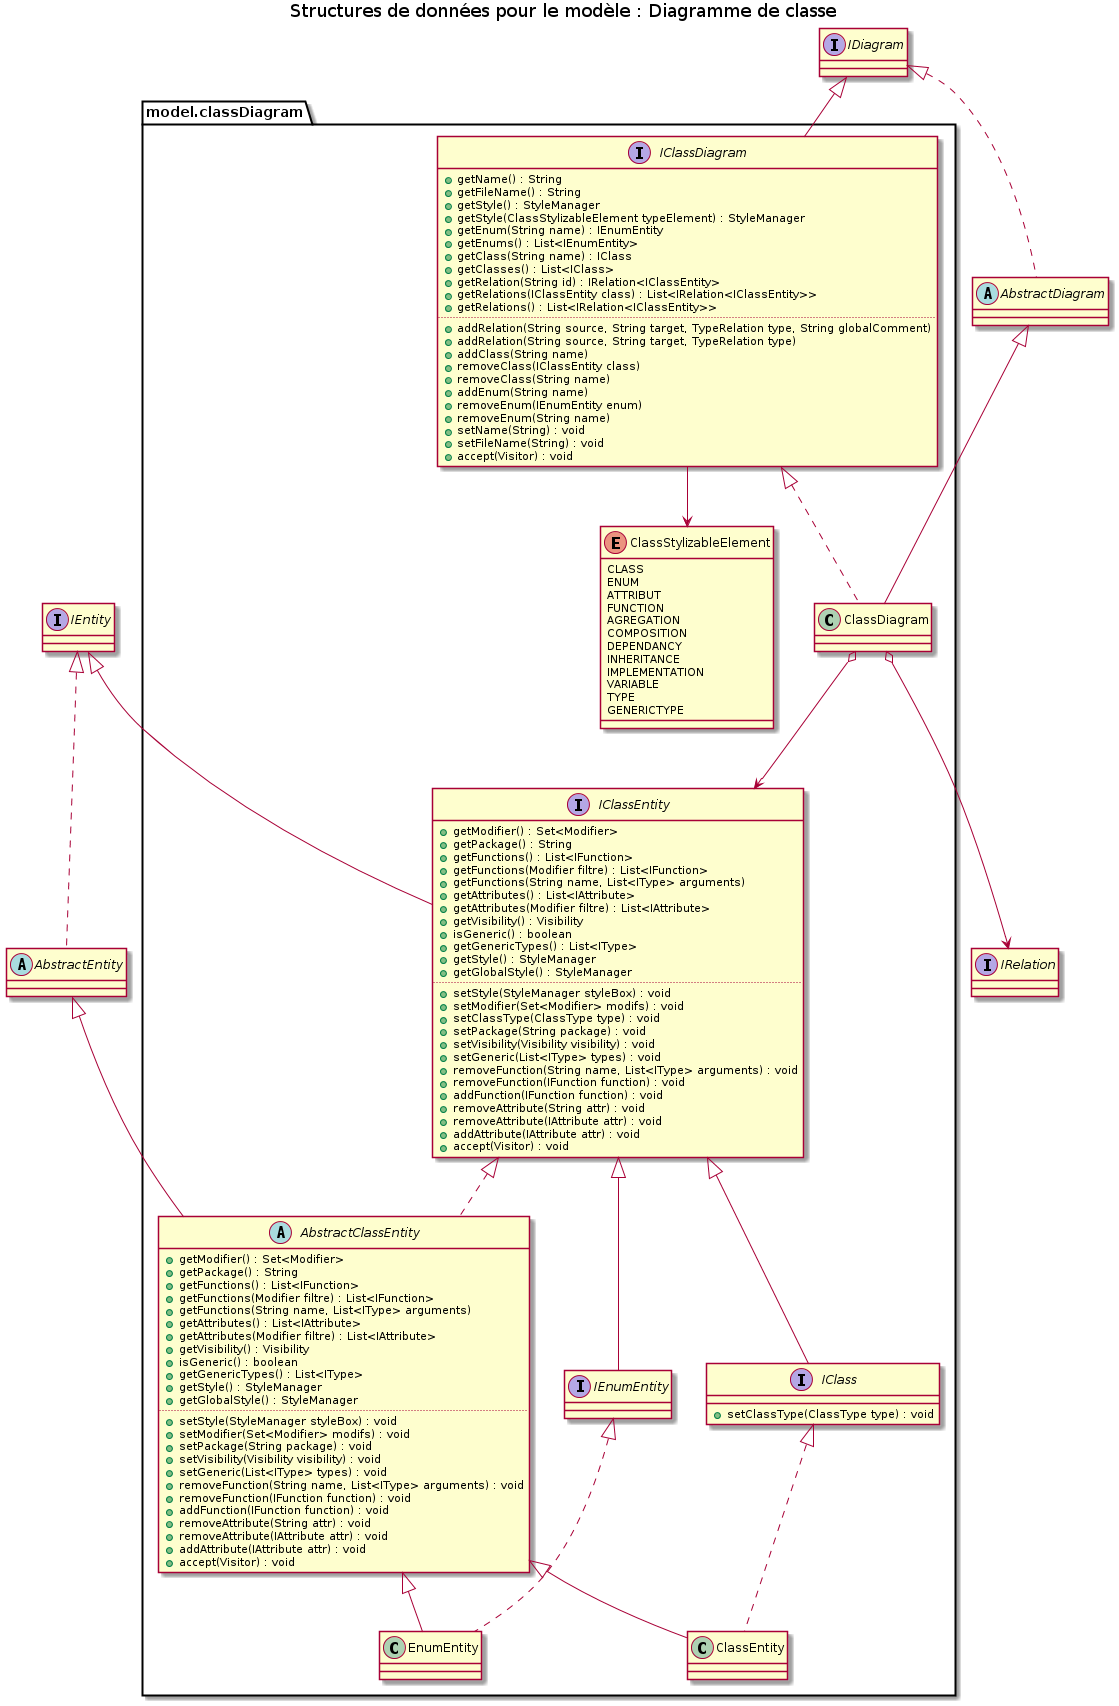
\includegraphics[width=\textwidth]{Image/classDiagramUp.png}
  \end{center}
  \begin{center}
      \includegraphics[width=12cm]{Image/classDiagramBottom.png}
  \end{center}
  Ce package contient le code pour stocker un diagramme de classe extrait à partir d'un fichier java. 
  A fortiori, il gère tout diagramme de classe en plantUml représentant un diagramme de classe valide en UML2.
  \subsubsection{sequenceDiagram}
  \begin{center}
      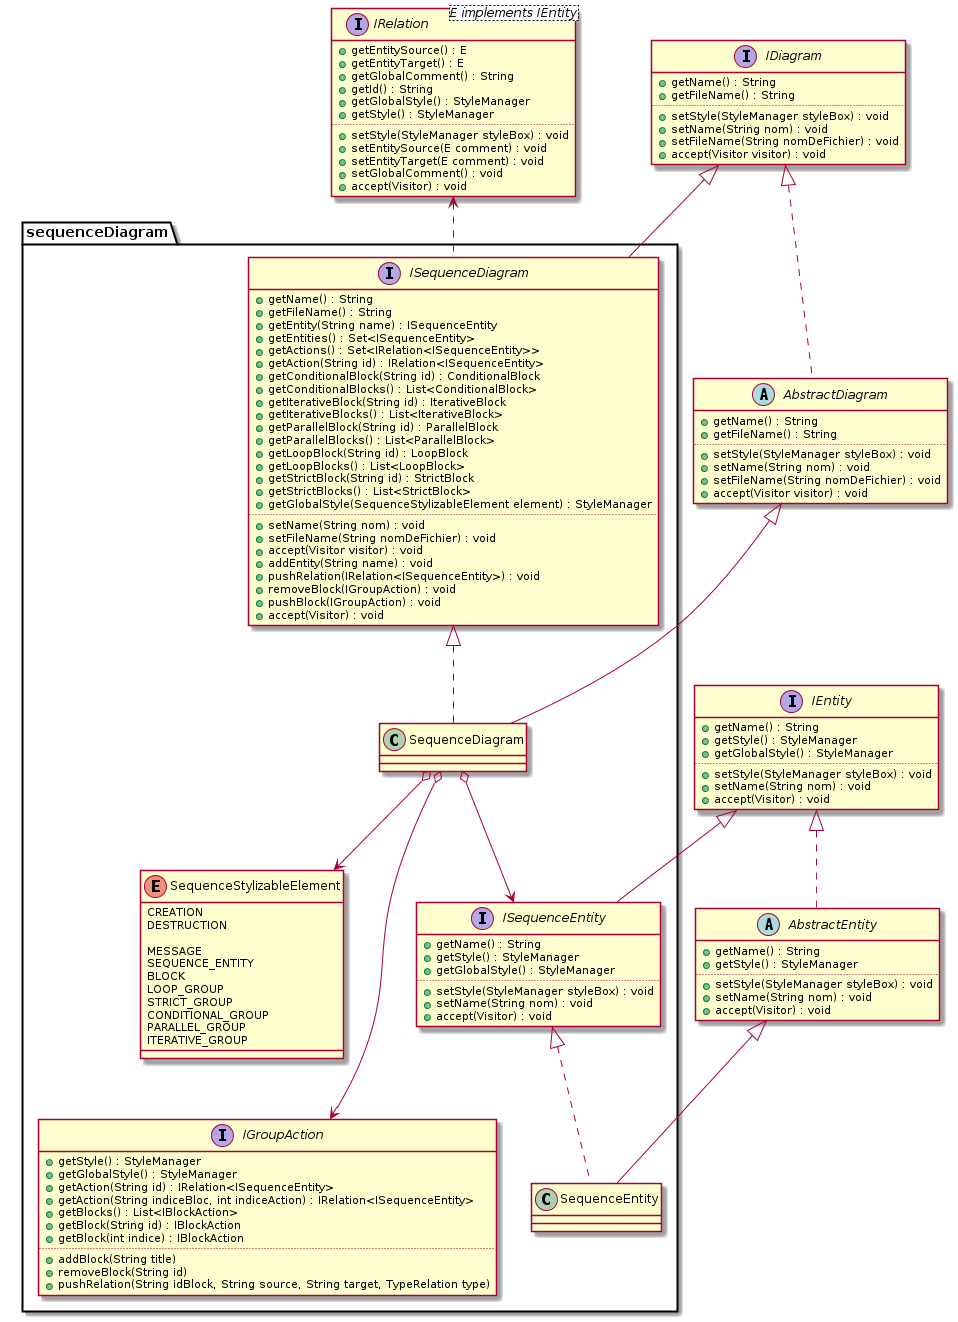
\includegraphics[width=\textwidth]{Image/SequenceDiag.png}
  \end{center}
  \begin{center}
      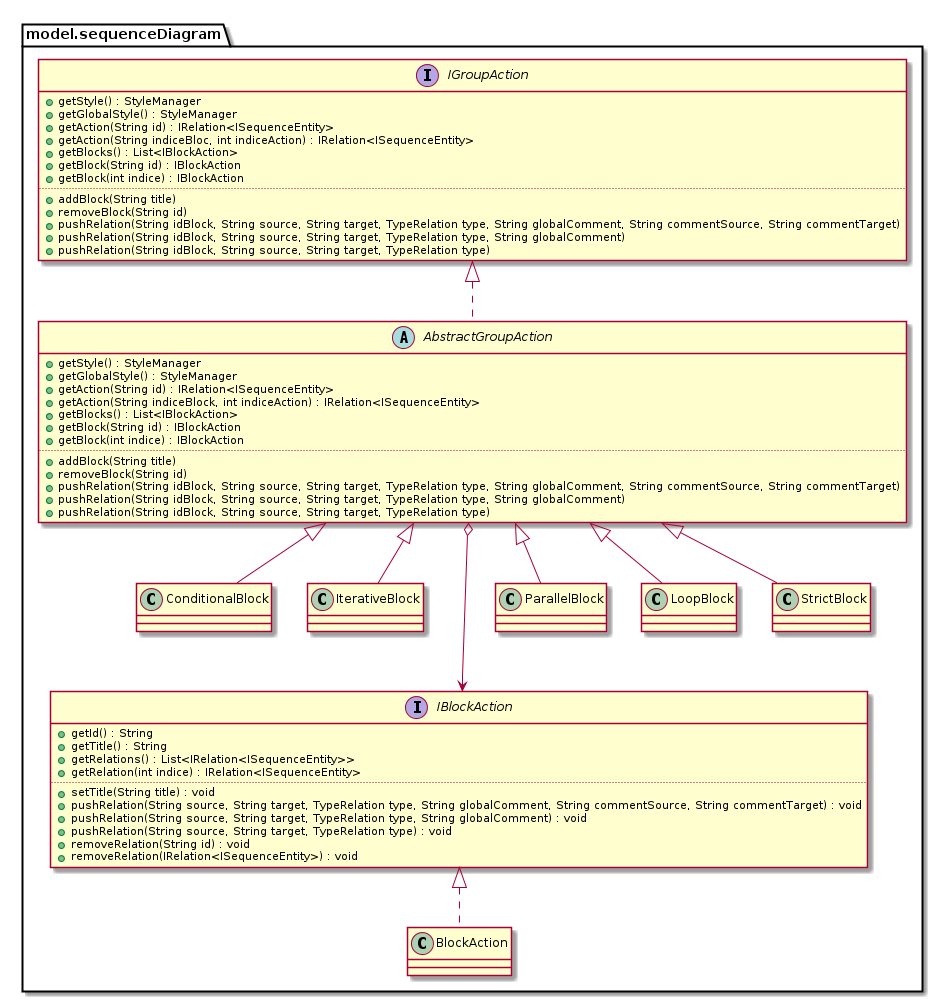
\includegraphics[width=\textwidth]{Image/SeqBlocksDiag.png}
  \end{center}
  Ce package contient le code pour stocker un diagramme de séquence. 
  Il gère tout diagramme de séquence en plantUml représentant un diagramme de séquence valide en UML2.
  \subsubsection{useCaseDiagram}
  \begin{center}
      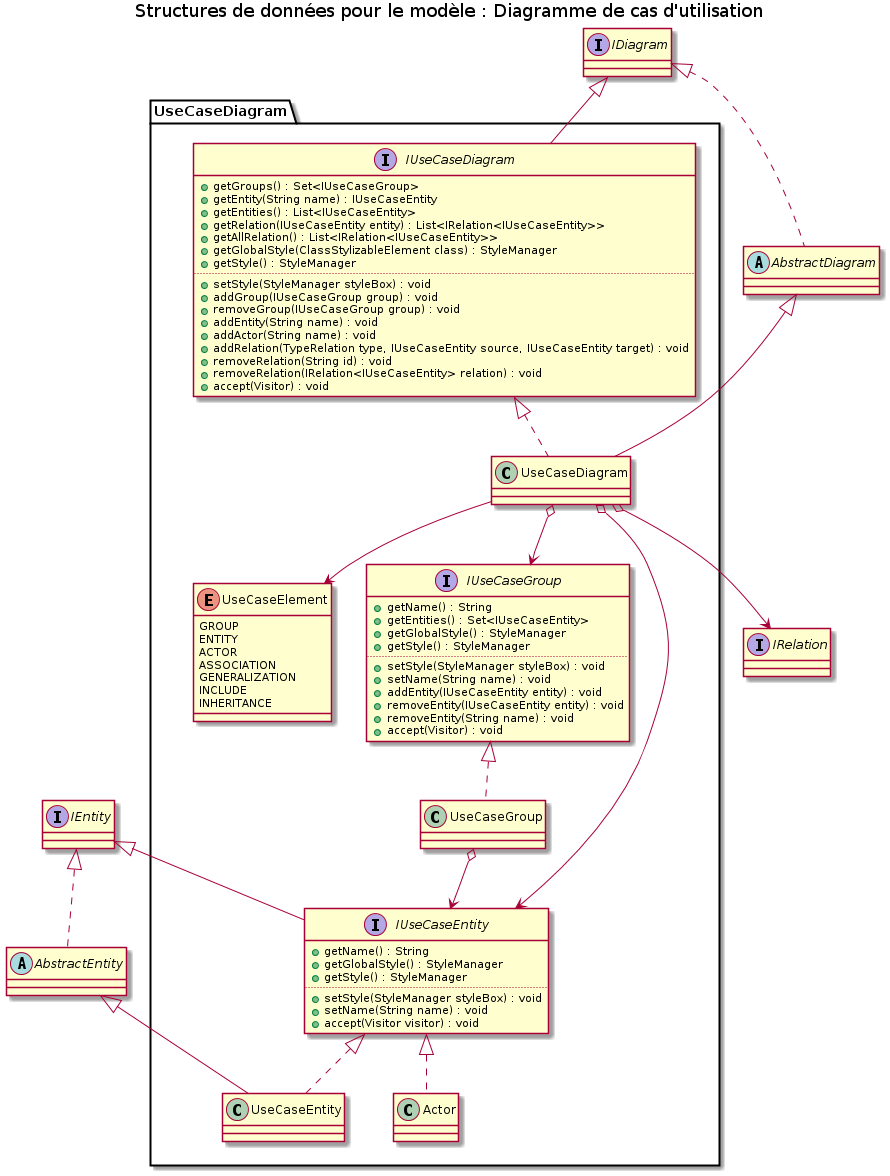
\includegraphics[width=\textwidth]{Image/UseCaseDiag.png}
  \end{center}
  Ce package contient le code pour stocker un diagramme de cas d'utilisation. 
  Il gère tout diagramme de cas d'utilisation en plantUml représentant un diagramme de séquence valide en UML2.
  \subsubsection{parser}
   Les imports
  \begin{center}
      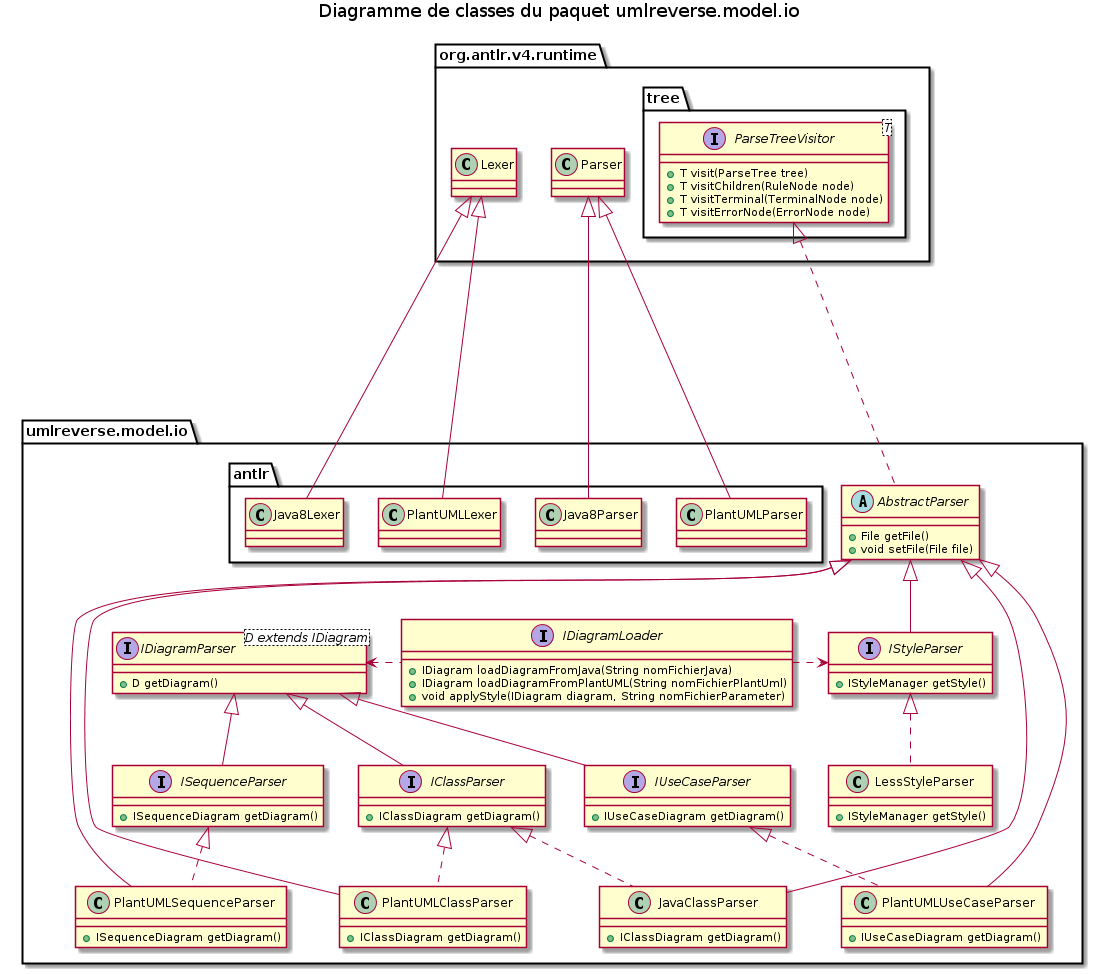
\includegraphics[width=\textwidth]{Image/parser.png}
  \end{center}
  Ce package contient les différents parsers qui seront utilisées pour extraire le style, le plantUml et le java.

  \subsection{ui}
  Ce package contient l'intégralité de la vue et des contrôleurs.
  \subsubsection{view}
  C'est dans ce package que se situe les différentes vues utilisées par l'application.
  \subsubsection{controllers}
  Ce package contient toutes les classes permettant la communication entre la vue et le modèle.
  \subsubsection{components}
  Les différents composants de l'ihm
  \begin{center}
      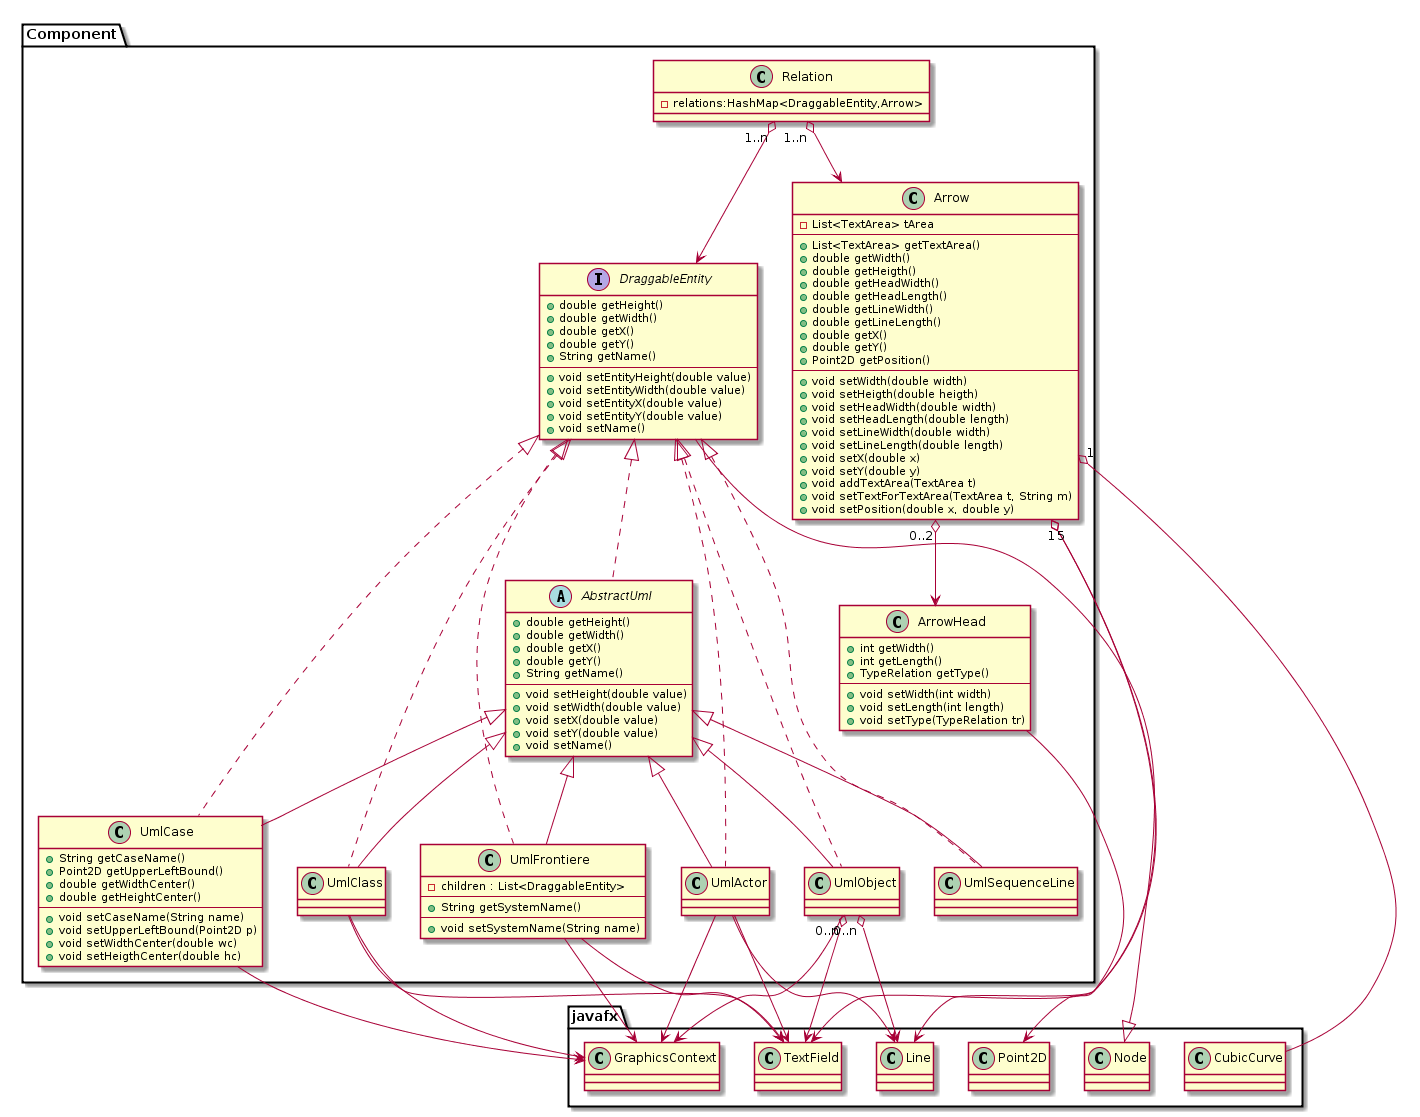
\includegraphics[width=\textwidth]{Image/Component.png}
  \end{center}
  Ce package contient les composants qui seront utilisées par la vue.
  
\section{}
\end{comment}

\end{document}
